\documentclass[a4paper]{article}
\usepackage[margin=3cm]{geometry}
\usepackage[french]{babel}
\usepackage[utf8]{inputenc}
\usepackage{amsmath}
\usepackage{graphicx}
\usepackage{schemabloc}
\usepackage[colorinlistoftodos]{todonotes}
\usepackage{hyperref}
\usepackage{float}


\title{Asservissement analogique en couple d'un moteur DC}

\author{Corentin Smith - Gabriel Samain}

\date{\today}

\begin{document}
\maketitle

\newpage
\tableofcontents
\newpage

\section{Préambule}

\subsection{Objectif}

L'objectif de ce TP est de réaliser l'asservissement analogique en couple / courant d'un moteur DC, le but final étant de simuler un effort par l'axe du moteur. \\
Pour cela, nous mettrons en pratique un schéma d'asservissement standard avec en entrée une tension de commande $U_{c}$, représentative d'un couple désiré, et en sortie mesurée une tension image de l'intensité traversant le moteur.

\subsection{Théorie}

L'équation électromécanique du moteur donne :
$$
C = k \cdot \Phi \cdot I \\
$$

Pour contrôler le couple du moteur, il suffit donc de réguler l'intensité du courant le traversant. Pour réaliser cela analogiquement, l'utilisation de tensions est nécessaire. C'est pourquoi une résistance de shunt est jointe au moteur afin d'avoir une tension image de l'intensité sans perturber le fonctionnement du circuit.

\section{Boucle d'asservissement}

\subsection{Schéma bloc}

\hfill \\
\begin{center}
\begin{tikzpicture}
\sbEntree{E}
\sbComp{comp}{E}
\sbRelier[$U_c$]{E}{comp}
\sbBloc{hach}{Hacheur}{comp}
\sbRelier[$\epsilon$]{comp}{hach}
\sbBloc{reg}{Régulateur}{hach}
\sbRelier[$U_h$]{hach}{reg}
\sbBloc{mot}{Moteur}{reg}
\sbRelier[$u$]{reg}{mot}
\sbSortie{S}{mot}
\sbRelier[$I$]{mot}{S}
\sbDecaleNoeudy[4]{S}{B}
\sbBlocr{shunt}{Shunt}{B}
\sbBlocrL{gainshunt}{$K_s$}{shunt}
\sbRelieryx{mot-S}{shunt}
\sbRelierxy[$U_m$]{gainshunt}{comp}
\end{tikzpicture}
\end{center}

\hfill \\\\
Les blocs assurent les fonctions suivantes :
\begin{description}
  \item[Hacheur] 	Transforme le signal $\epsilon$ en PWM grâce à un comparateur à hysterésis et un signal triangle
  \item[Régulateur] Duplique et inverse le signal précédent puis l'injecte dans un pont en H
  \item[Moteur] 	Le système à contrôler
  \item[Shunt] 		Une résistance de shunt permet de “lire le courant” sous forme de tension
  \item[K$_{s}$]	Un gain permet d'ajuster la tension lue pour l'adaptée à l'entrée 
\end{description}

\hfill \\
Nota : L'utilisation d'un gain simple $K_{s}$ est possible car il existe une relation linéaire entre tension lue aux bornes de la résistance de shunt et la tension de commande, ce qui sera montré plus bas.

\subsection{Schéma électrique}

La première partie du circuit fait la différence du signal de commande continu $U_{c}$ et de la tension mesurée aux bornes de la résistance de shunt (en boucle ouverte, cette tension est nulle). Cette différence $\epsilon$ est ensuite transformée en PWM proportionnel grâce à un comparateur à hysteresis et à un signal triangulaire.

Ce signal est ensuite dupliqué et inversé par un simple amplificateur opérationnel inverseur. Ces deux signaux sont injectés dans un pont en H qui permet de réaliser une amplification de puissance de la PWM. La tension efficace de cette PWM est proportionnelle à la largeur d'impulsion, et la vitesse de rotation du moteur est donc reliée directement à la tension de commande.

\begin{figure}[H]
\centering
	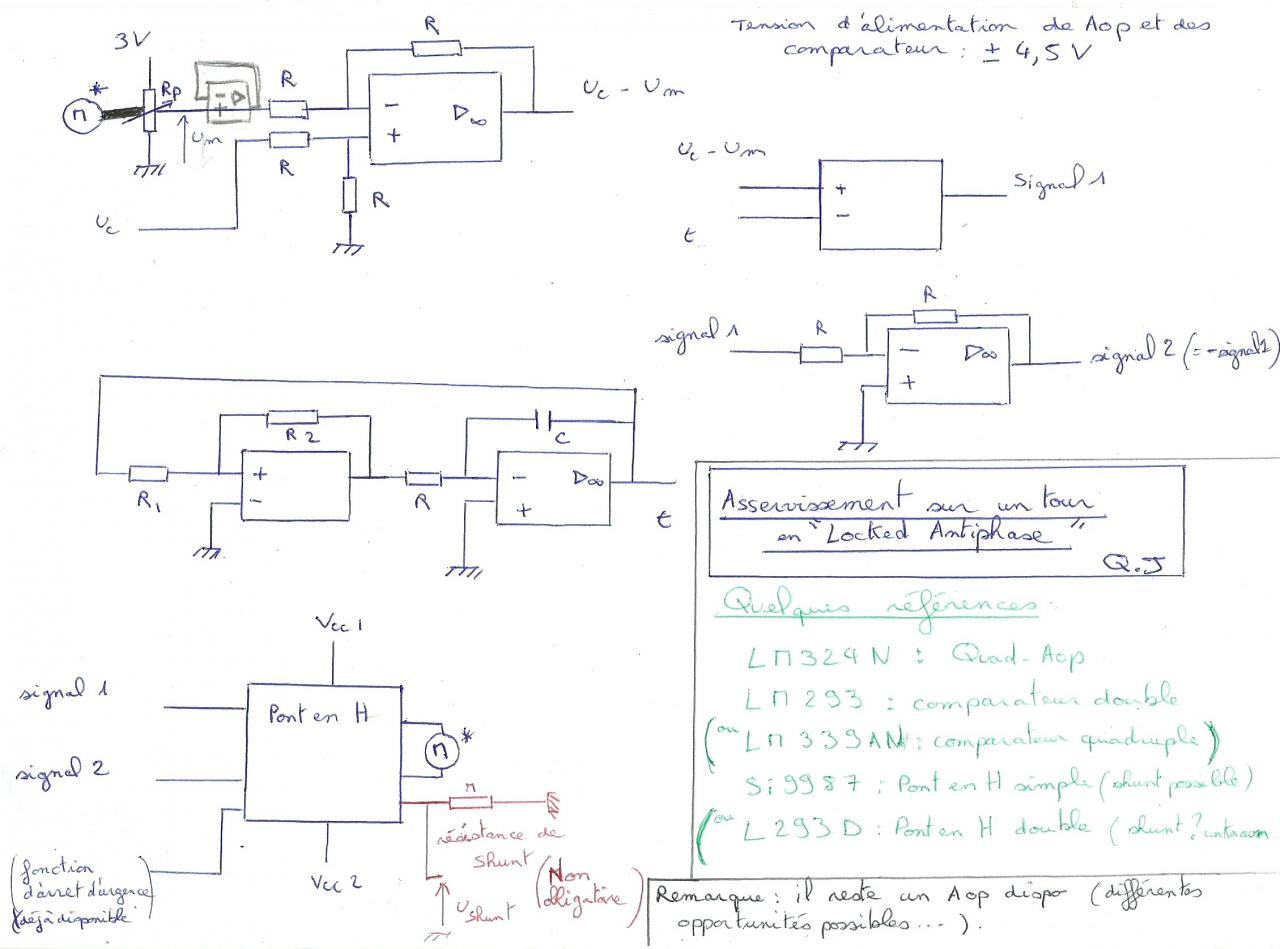
\includegraphics[width=1\textwidth]{schema.png}
	\caption{Schéma électrique en boucle ouverte}
\end{figure}


\begin{figure}[H]
\centering
	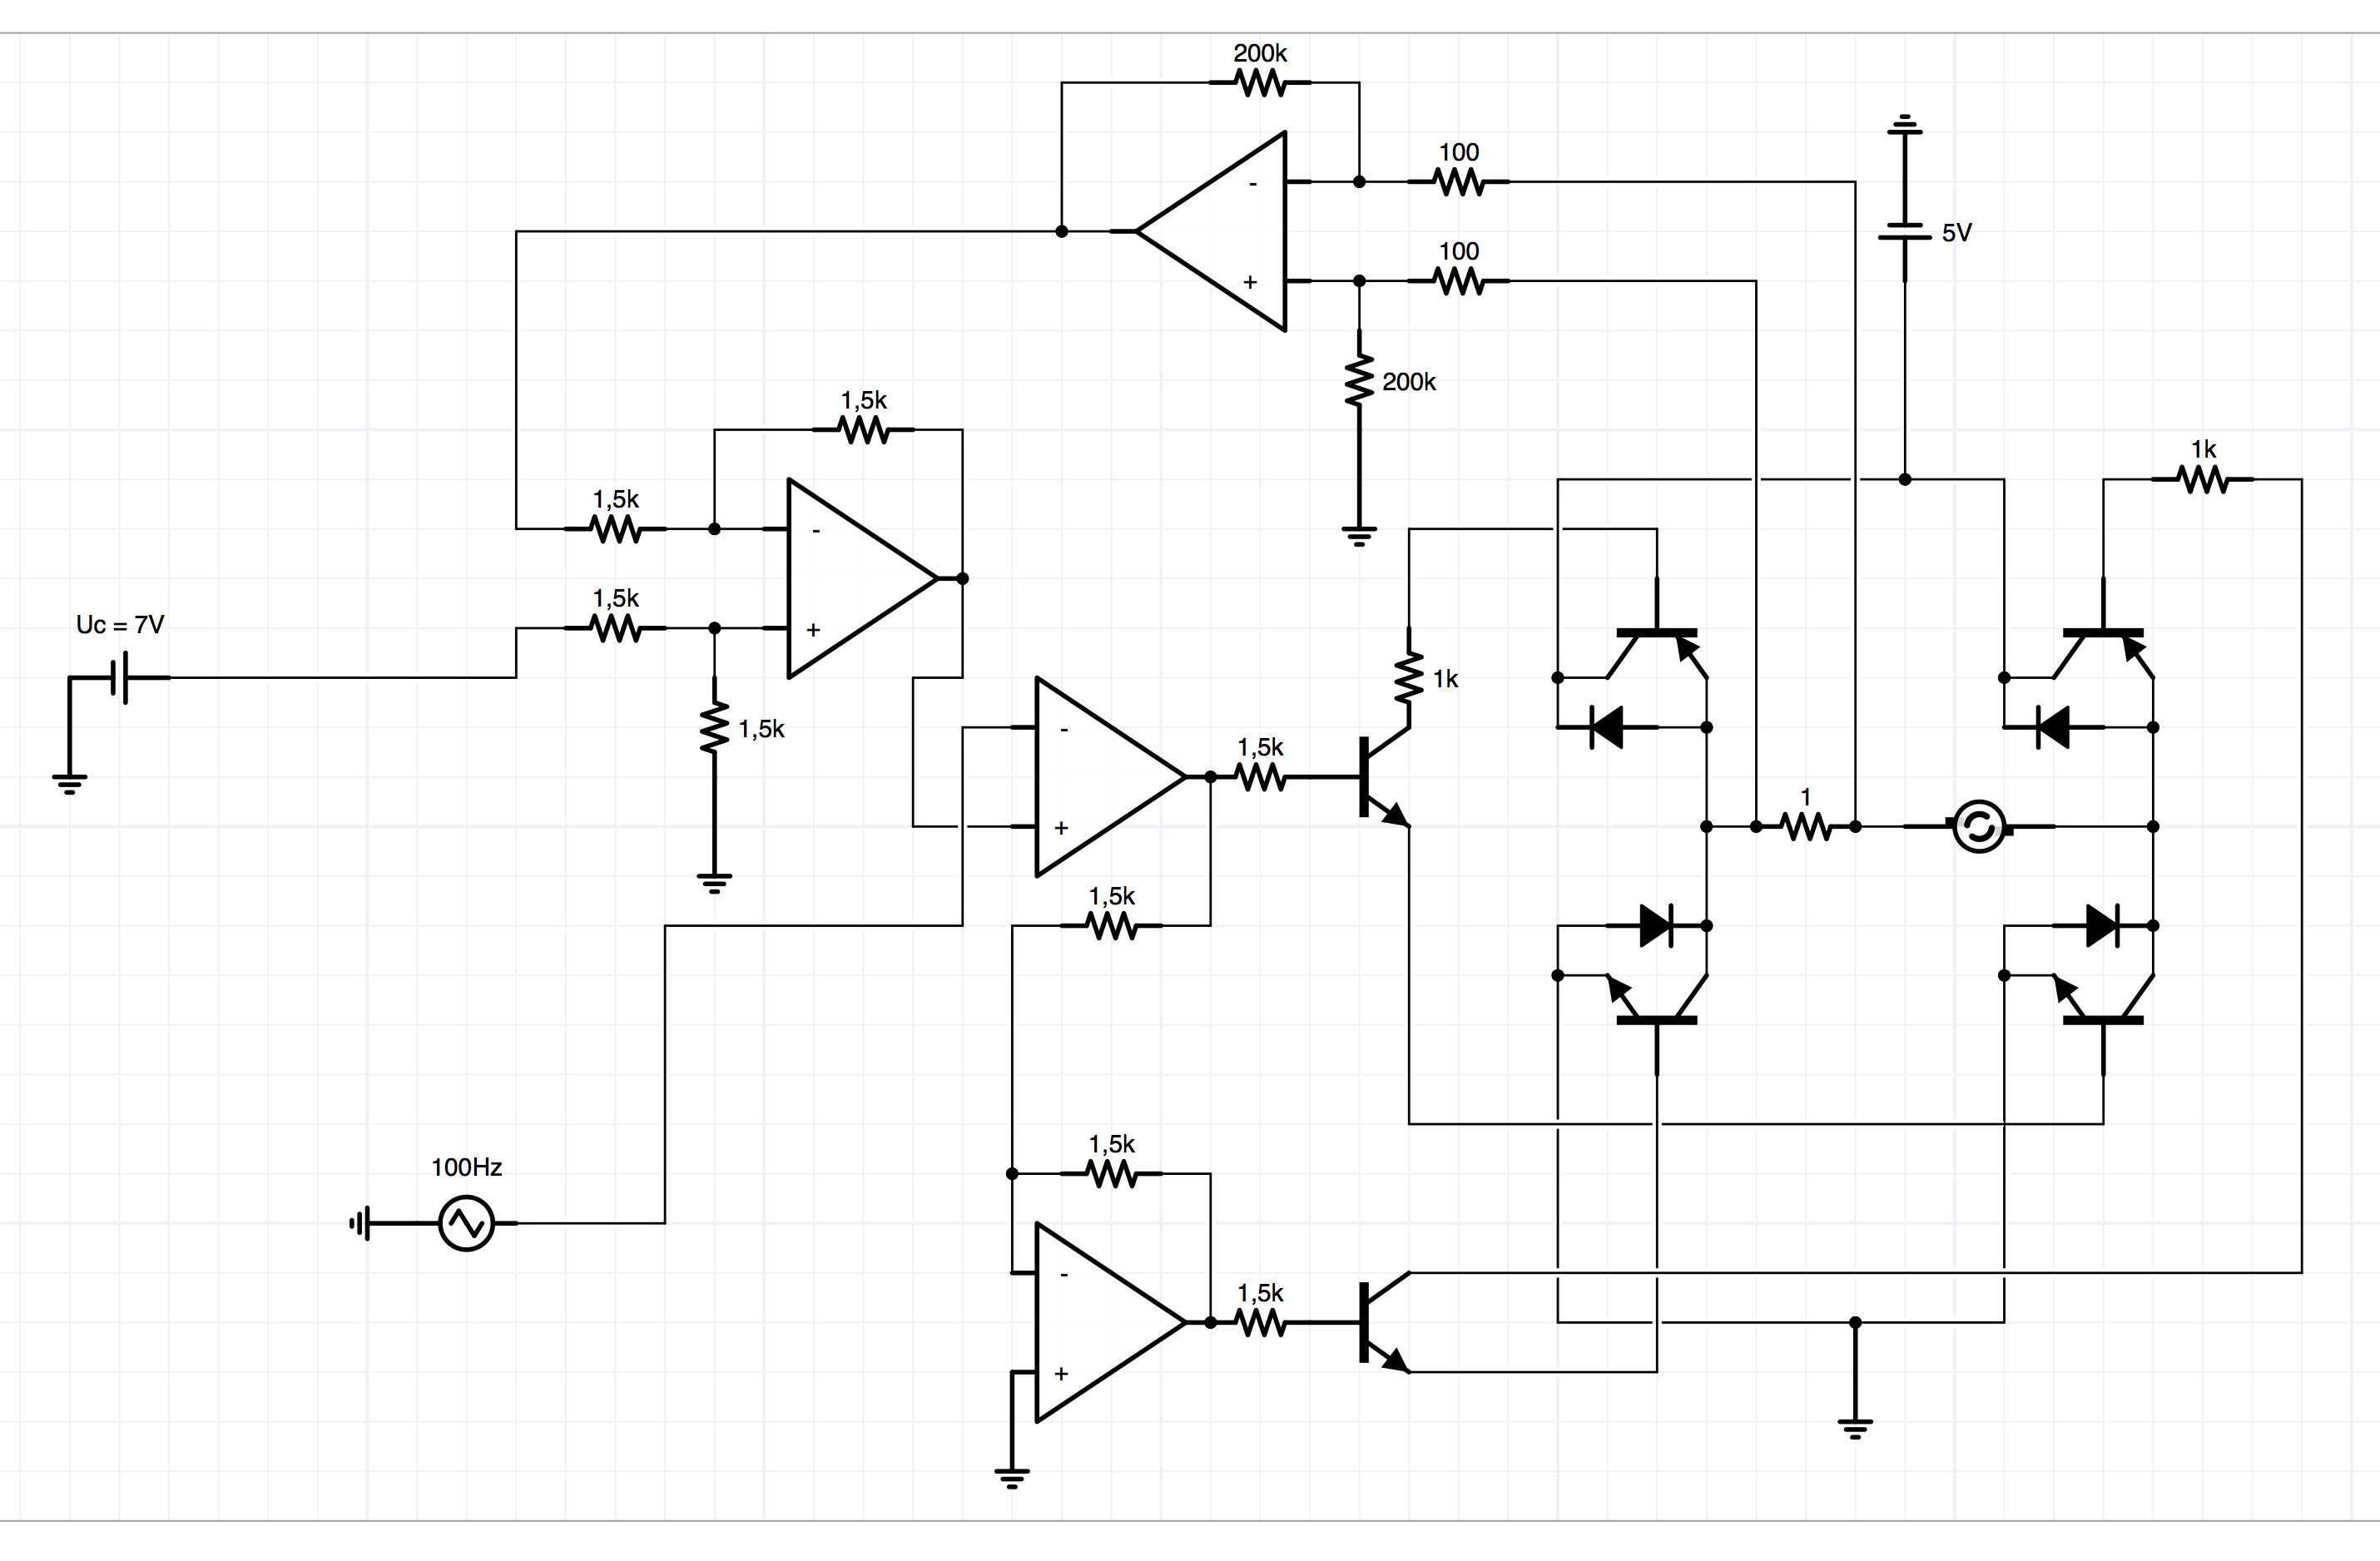
\includegraphics[width=1\textwidth]{schema_boucle.png}
	\caption{Schéma électrique en boucle fermée}
\end{figure}


\subsection{Choix des composants}

Nous avions prévu de réaliser le circuit avec un pont en H de TI, le LMD18245T \href{http://www.ti.com/lit/ds/symlink/lmd18245.pdf}{[datasheet]}, mais nous n'avons pas réussi à le faire fonctionner correctement et nous avons décidé de réaliser le pont en H à la main, le circuit étant assez simple.

Les transistors que nous avons choisis sont des transistors de moyenne puissance, les BD237 (NPN) et BD238 (PNP) \href{http://www.onsemi.com/pub_link/Collateral/BD237-D.PDF}{[datasheet]}.

Les amplificateurs opérationnels sont des LM324AN \href{https://www.fairchildsemi.com/datasheets/LM/LM324.pdf}{[datasheet]}. Nous avons également utilisé les amplificateurs opérationnels en tant que comparateurs afin de limiter le nombre de composants.\\

Afin de déterminer la valeur du gain $K_s$ nécessaire en sortie de la boucle (entre la résistance de shunt et l'entrée du sommateur), nous avons réalisé une série de mesures de la tension aux bornes de la résistance de shunt.

On obtient une courbe linéaire qui nous permet de déterminer la valeur de $K_s = 1/0.0166 = 60.24$. On a donc choisi pour les résistances $56k\Omega + 3.9k\Omega$ et $1k\Omega$ pour obtenir un rapport d'environ 60. 

Par soucis de simplicité, nous avons décider de ne pas compenser l'offset de $0.0066V$, ce qui influe peu sur l'interprétation des résultats.


\begin{figure}[H]
	\centering
	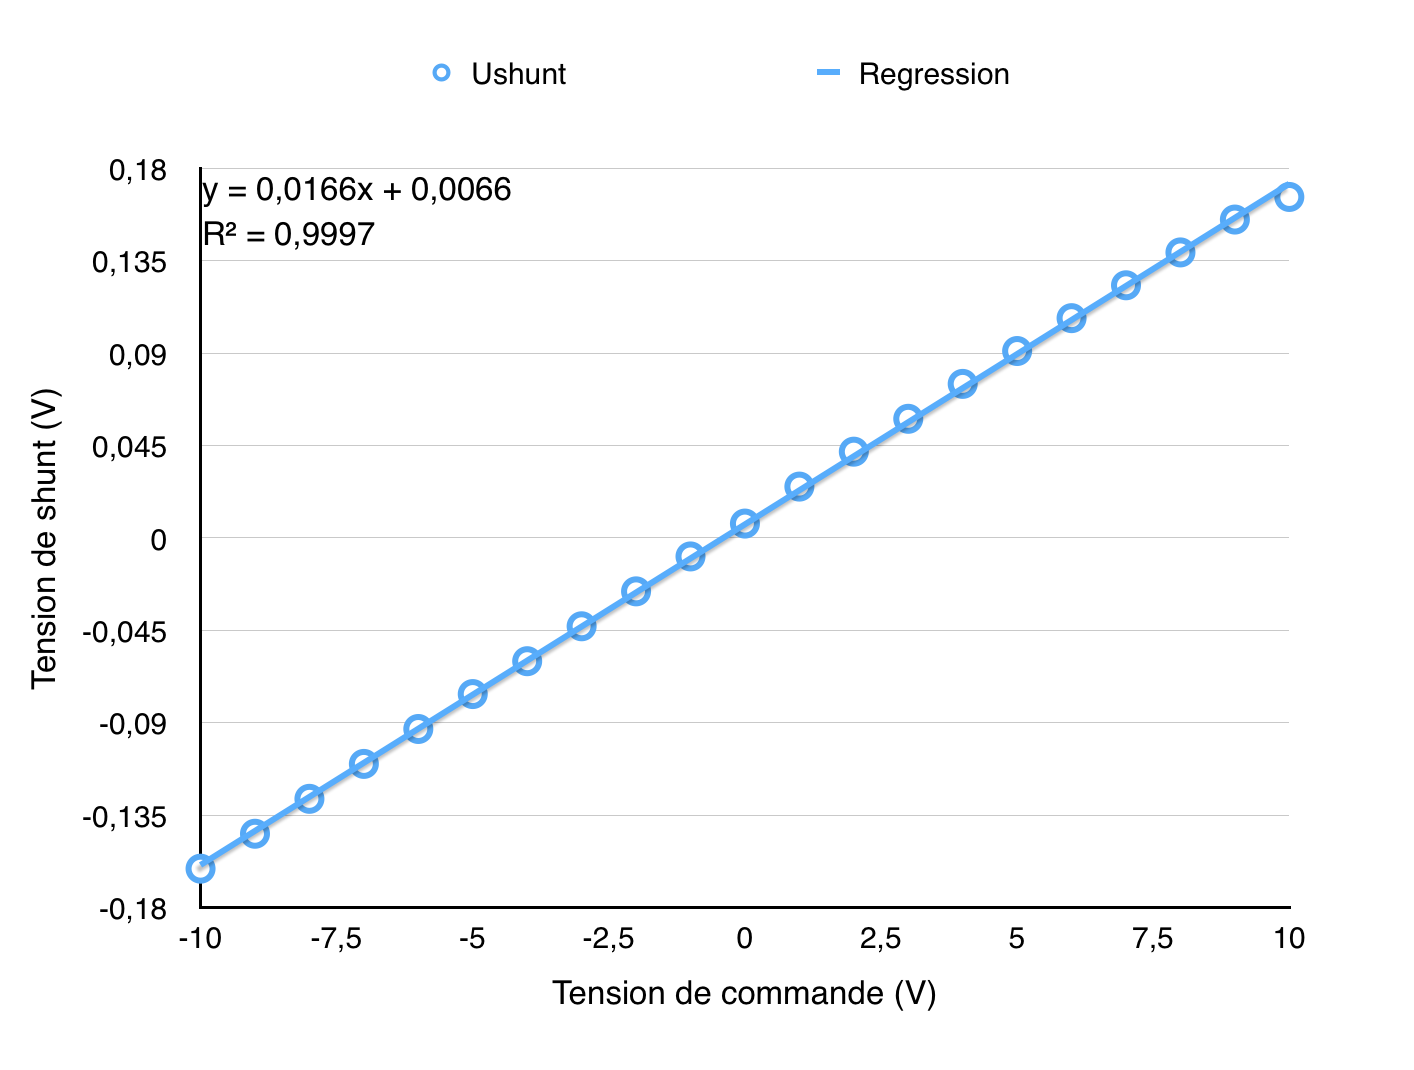
\includegraphics[width=1\textwidth]{graph_shunt.png}
	\caption{Relation entre commande et tension aux bornes de la résistance de shunt}
\end{figure}



\section{Réalisation}

\subsection{Simulation}

La simulation théorique du circuit se fait à l'aide du logiciel iCircuit qui permet une visualisation en temps réel des grandeurs physiques caractéristiques de chaque composant du circuit.

Pour ce qui est du bouclage, le modèle de moteur inclus dans le logiciel n'étant pas très réaliste, nous n'avons pas réalisé de simulation.

Nous pouvons voir à travers les résultats suivants que la tension de commande permet en théorie un contrôle précis de la vitesse de rotation du moteur mais aussi de l'intensité moyenne à laquelle il est soumis. En bouclant via la tension de shunt, image de cette intensité, un contrôle du couple est donc possible.

Nota : Toutes les courbes suivantes représentent les grandeurs physiques aux bornes du moteur.

\begin{figure}[H]
	\centering
	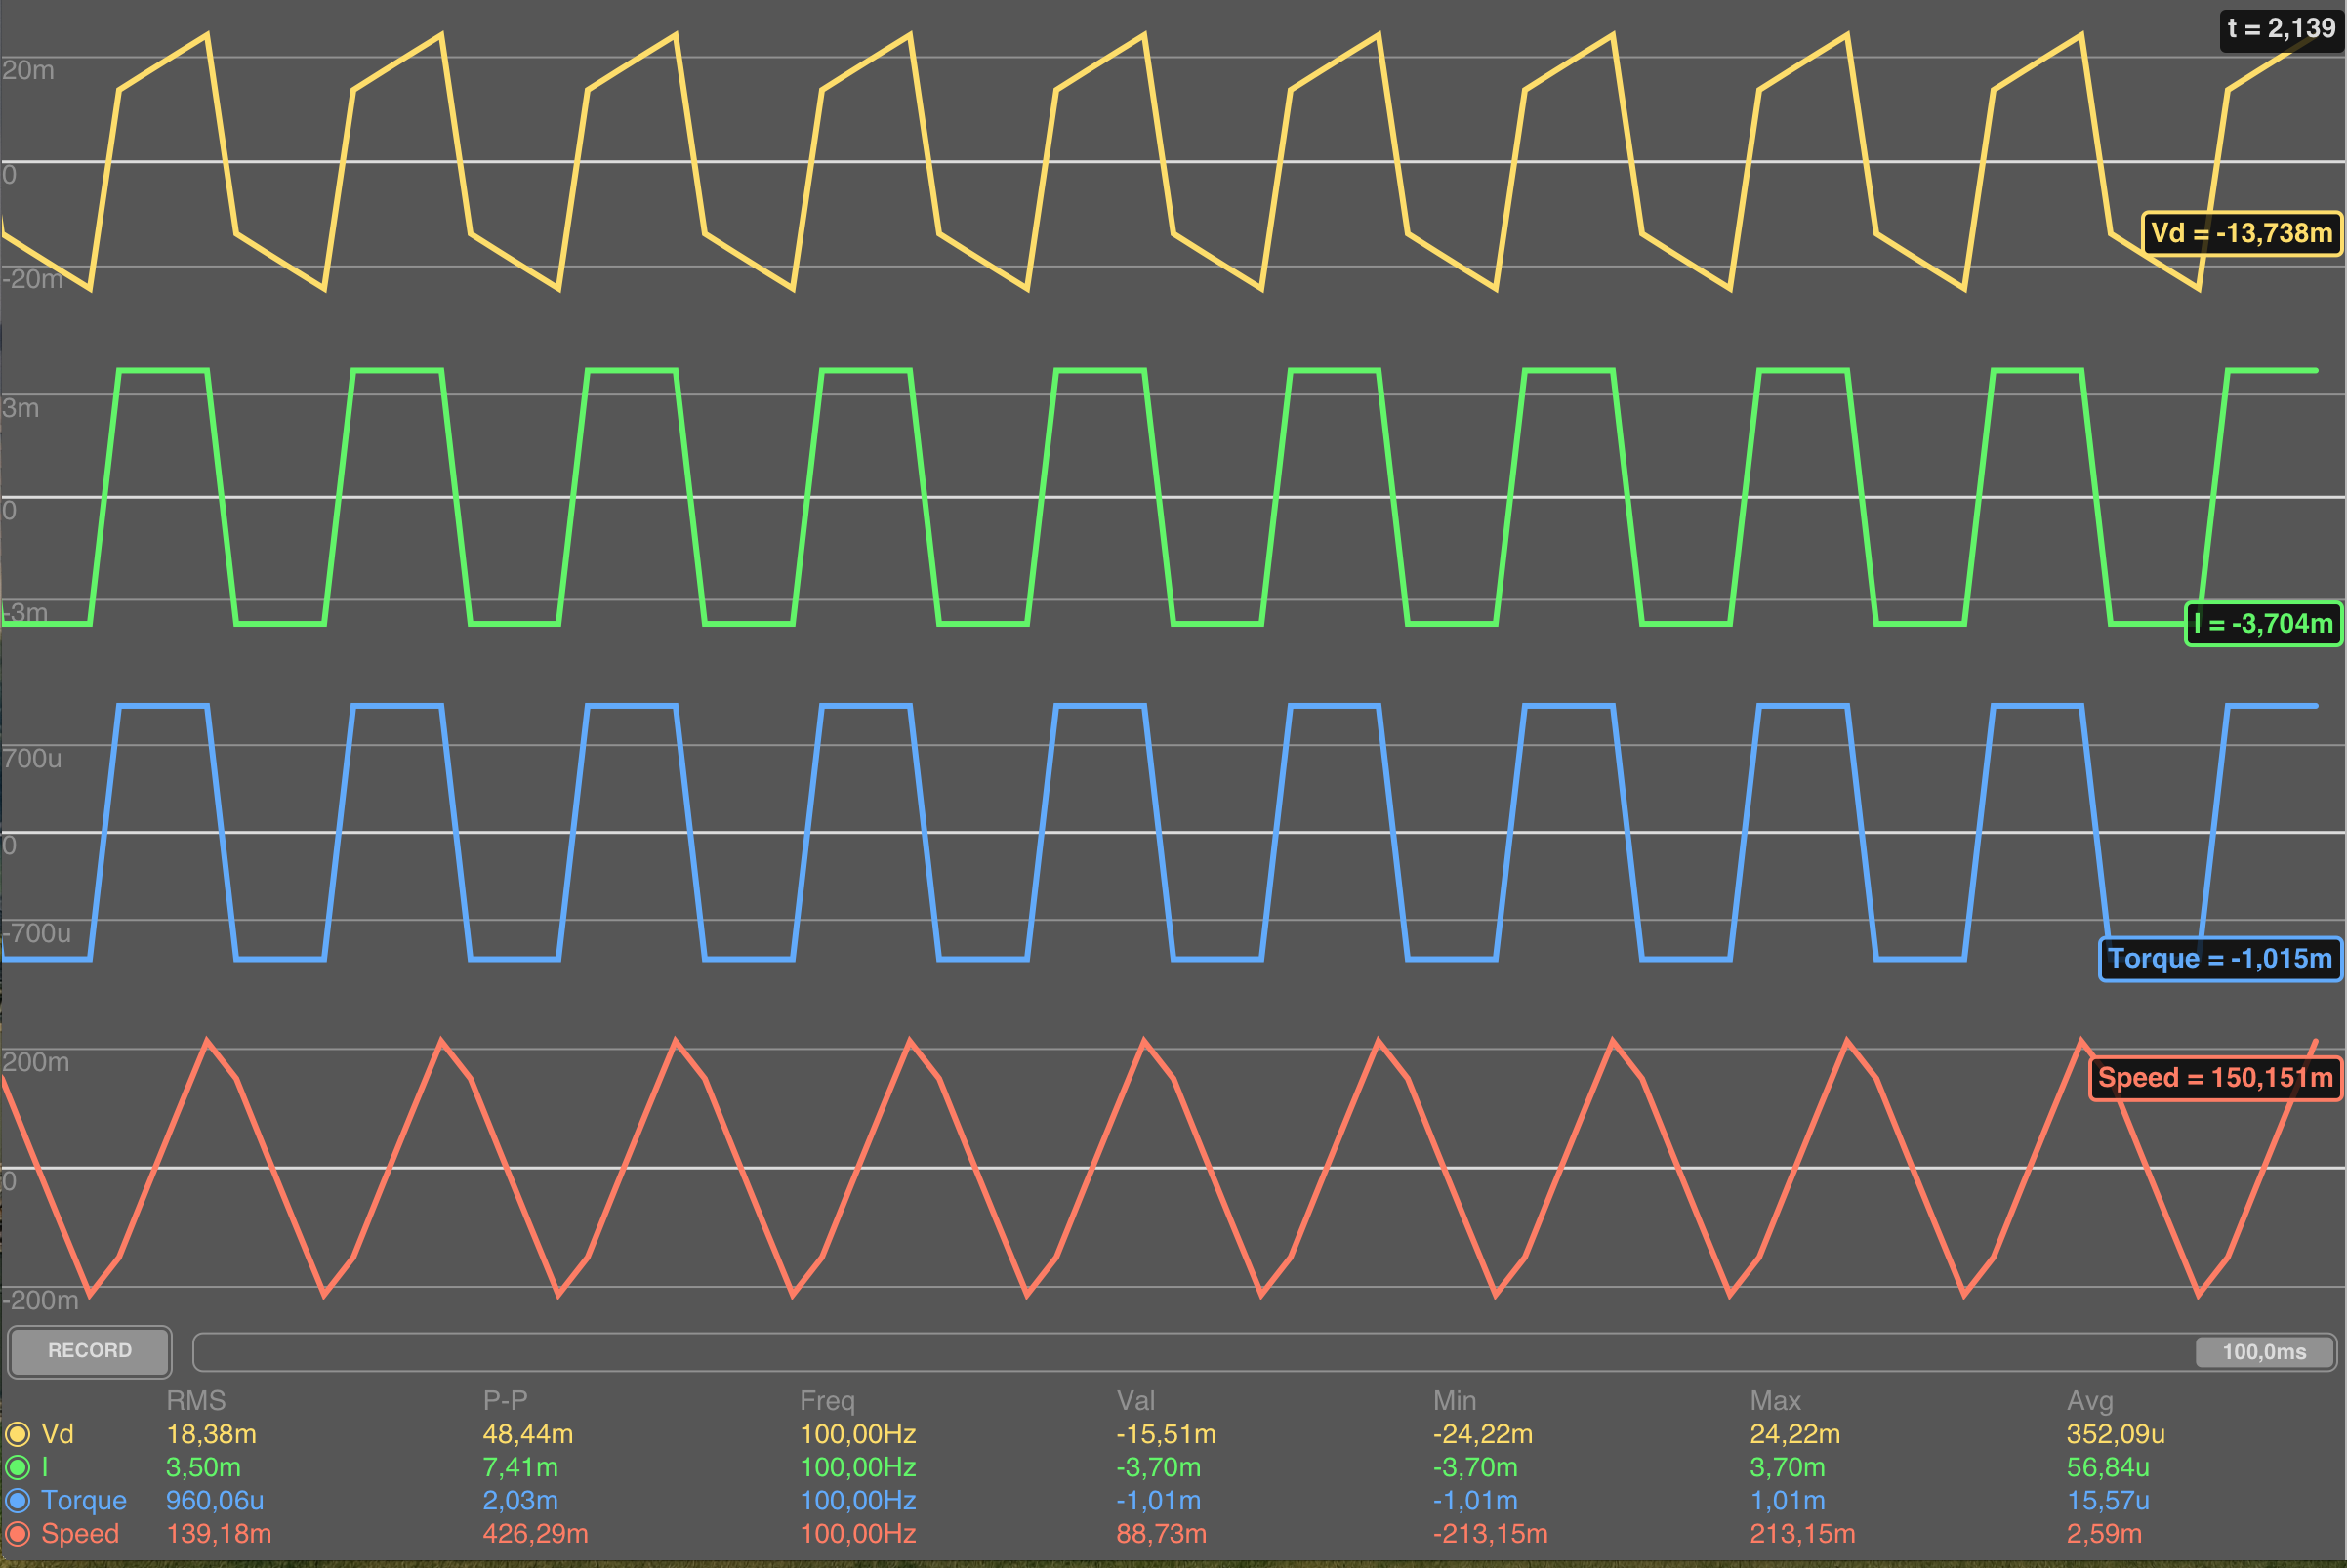
\includegraphics[width=1\textwidth]{simu0v}
	\caption{Simulation (boucle ouverte) avec une commande de 0V}
\end{figure}
\begin{figure}[H]
	\centering
	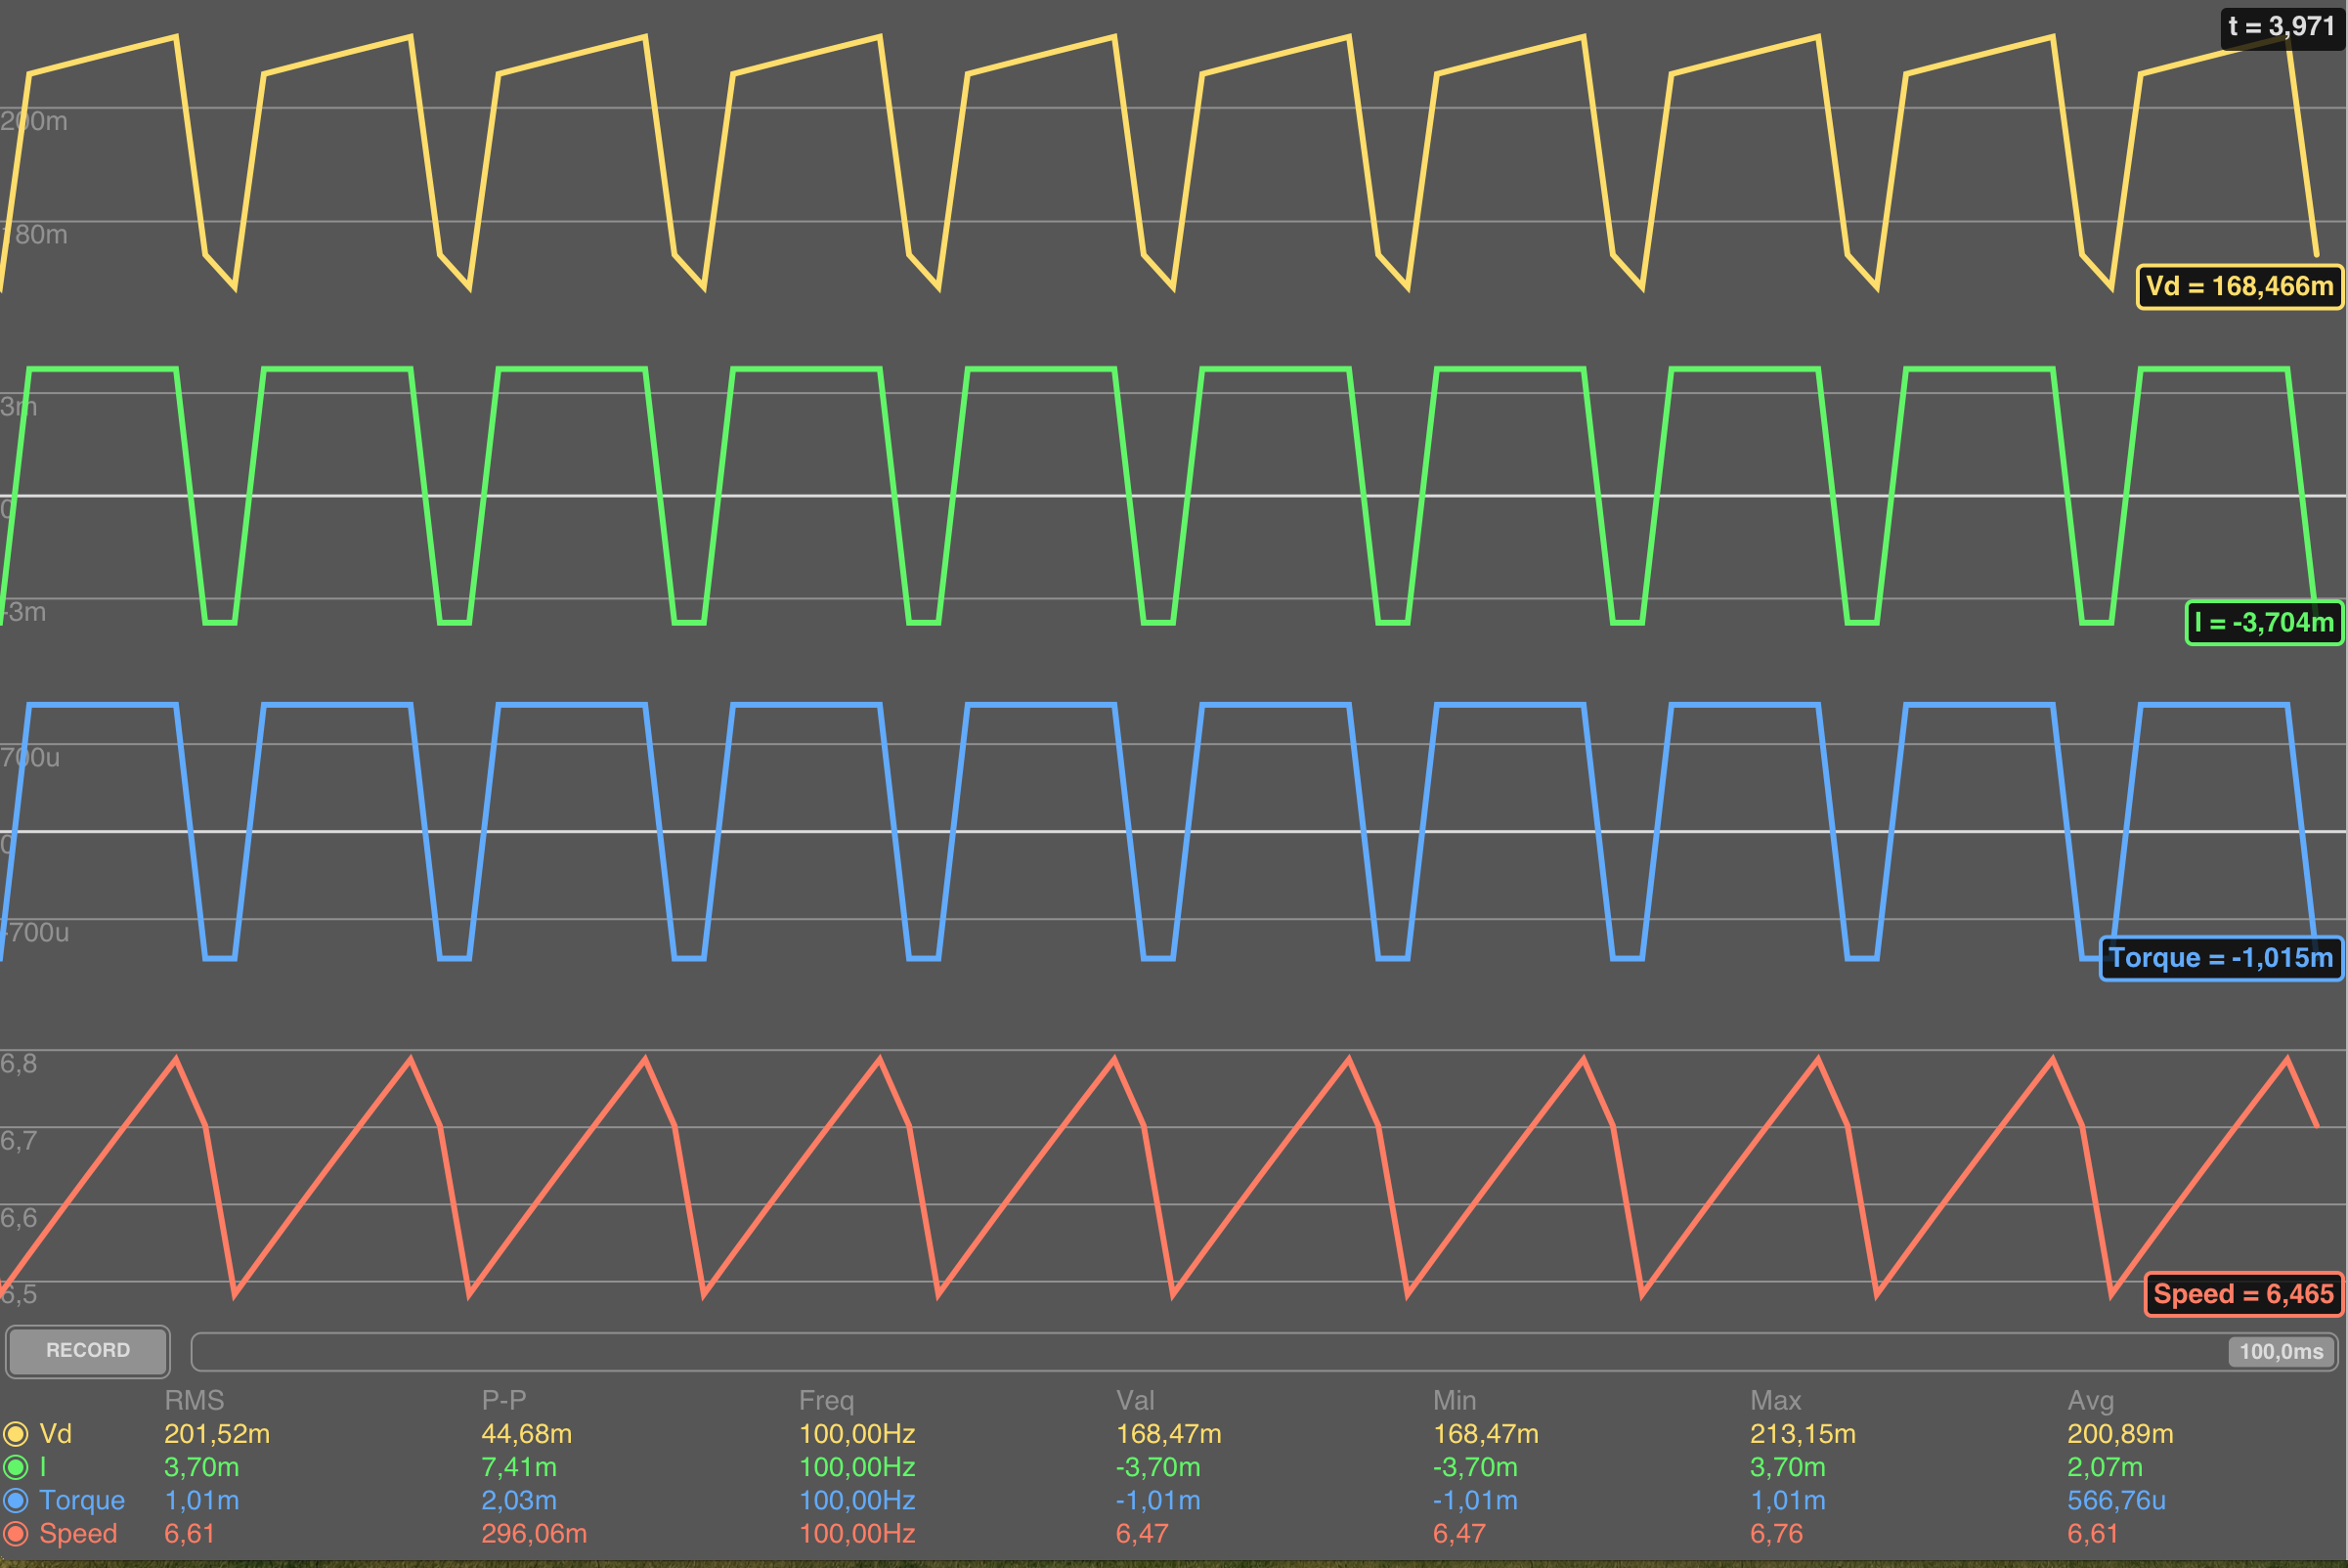
\includegraphics[width=1\textwidth]{simu7v}
	\caption{Simulation (boucle ouverte) avec une commande de 7V}
\end{figure}
\begin{figure}[H]
	\centering
	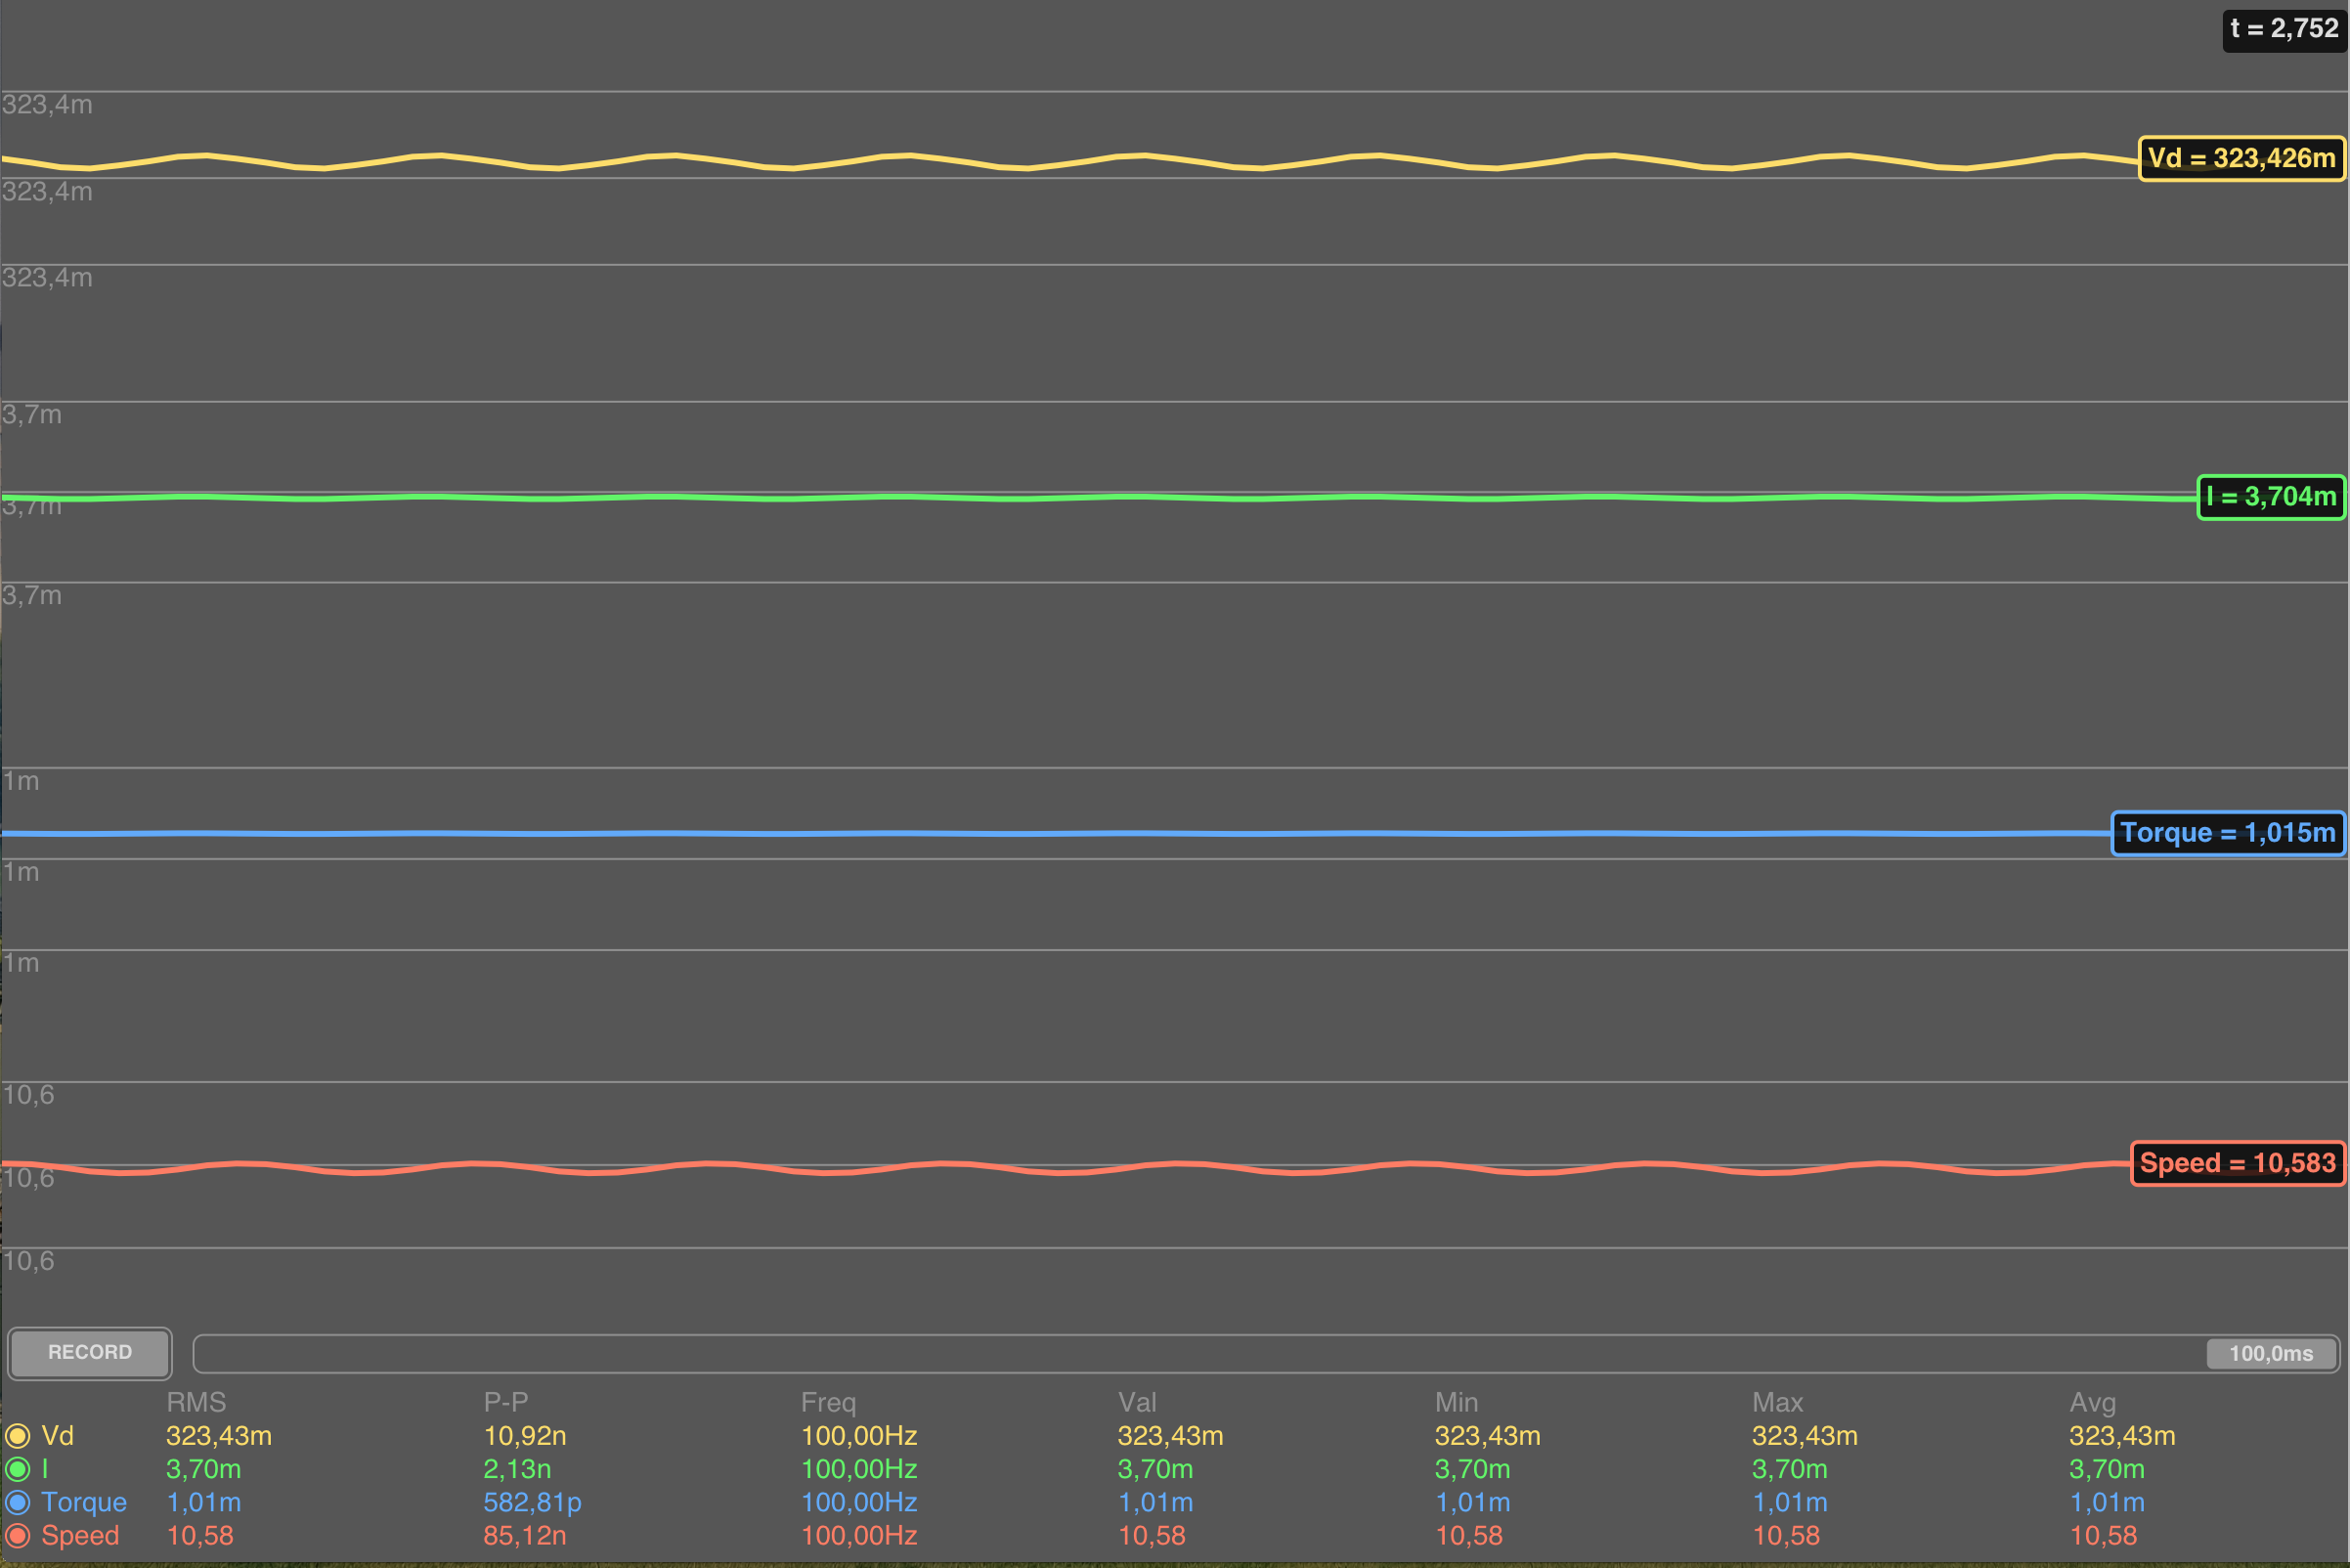
\includegraphics[width=1\textwidth]{simu15v}
	\caption{Simulation (boucle ouverte) avec une commande de 15V}
\end{figure}

\subsection{Circuit}

La majorité des problèmes rencontrés lors de la réalisation de ce circuit venaient du pont en H : mauvais branchements, étiquetage des transistors erroné, surchauffe des transistors, etc.

Comme montré sur la photo suivante, nous avons choisi de refroidir les transistors en les fixant sur des plaques d'aluminium et en réduisant la tension d'alimentation du pont en H à 10V. La méthode s'est avérée très efficace.

Une plaque de carton plume a été fixée sur l'axe du moteur afin d'avoir une meilleure appréciation du couple du moteur.

\begin{figure}[H]
  \centering
    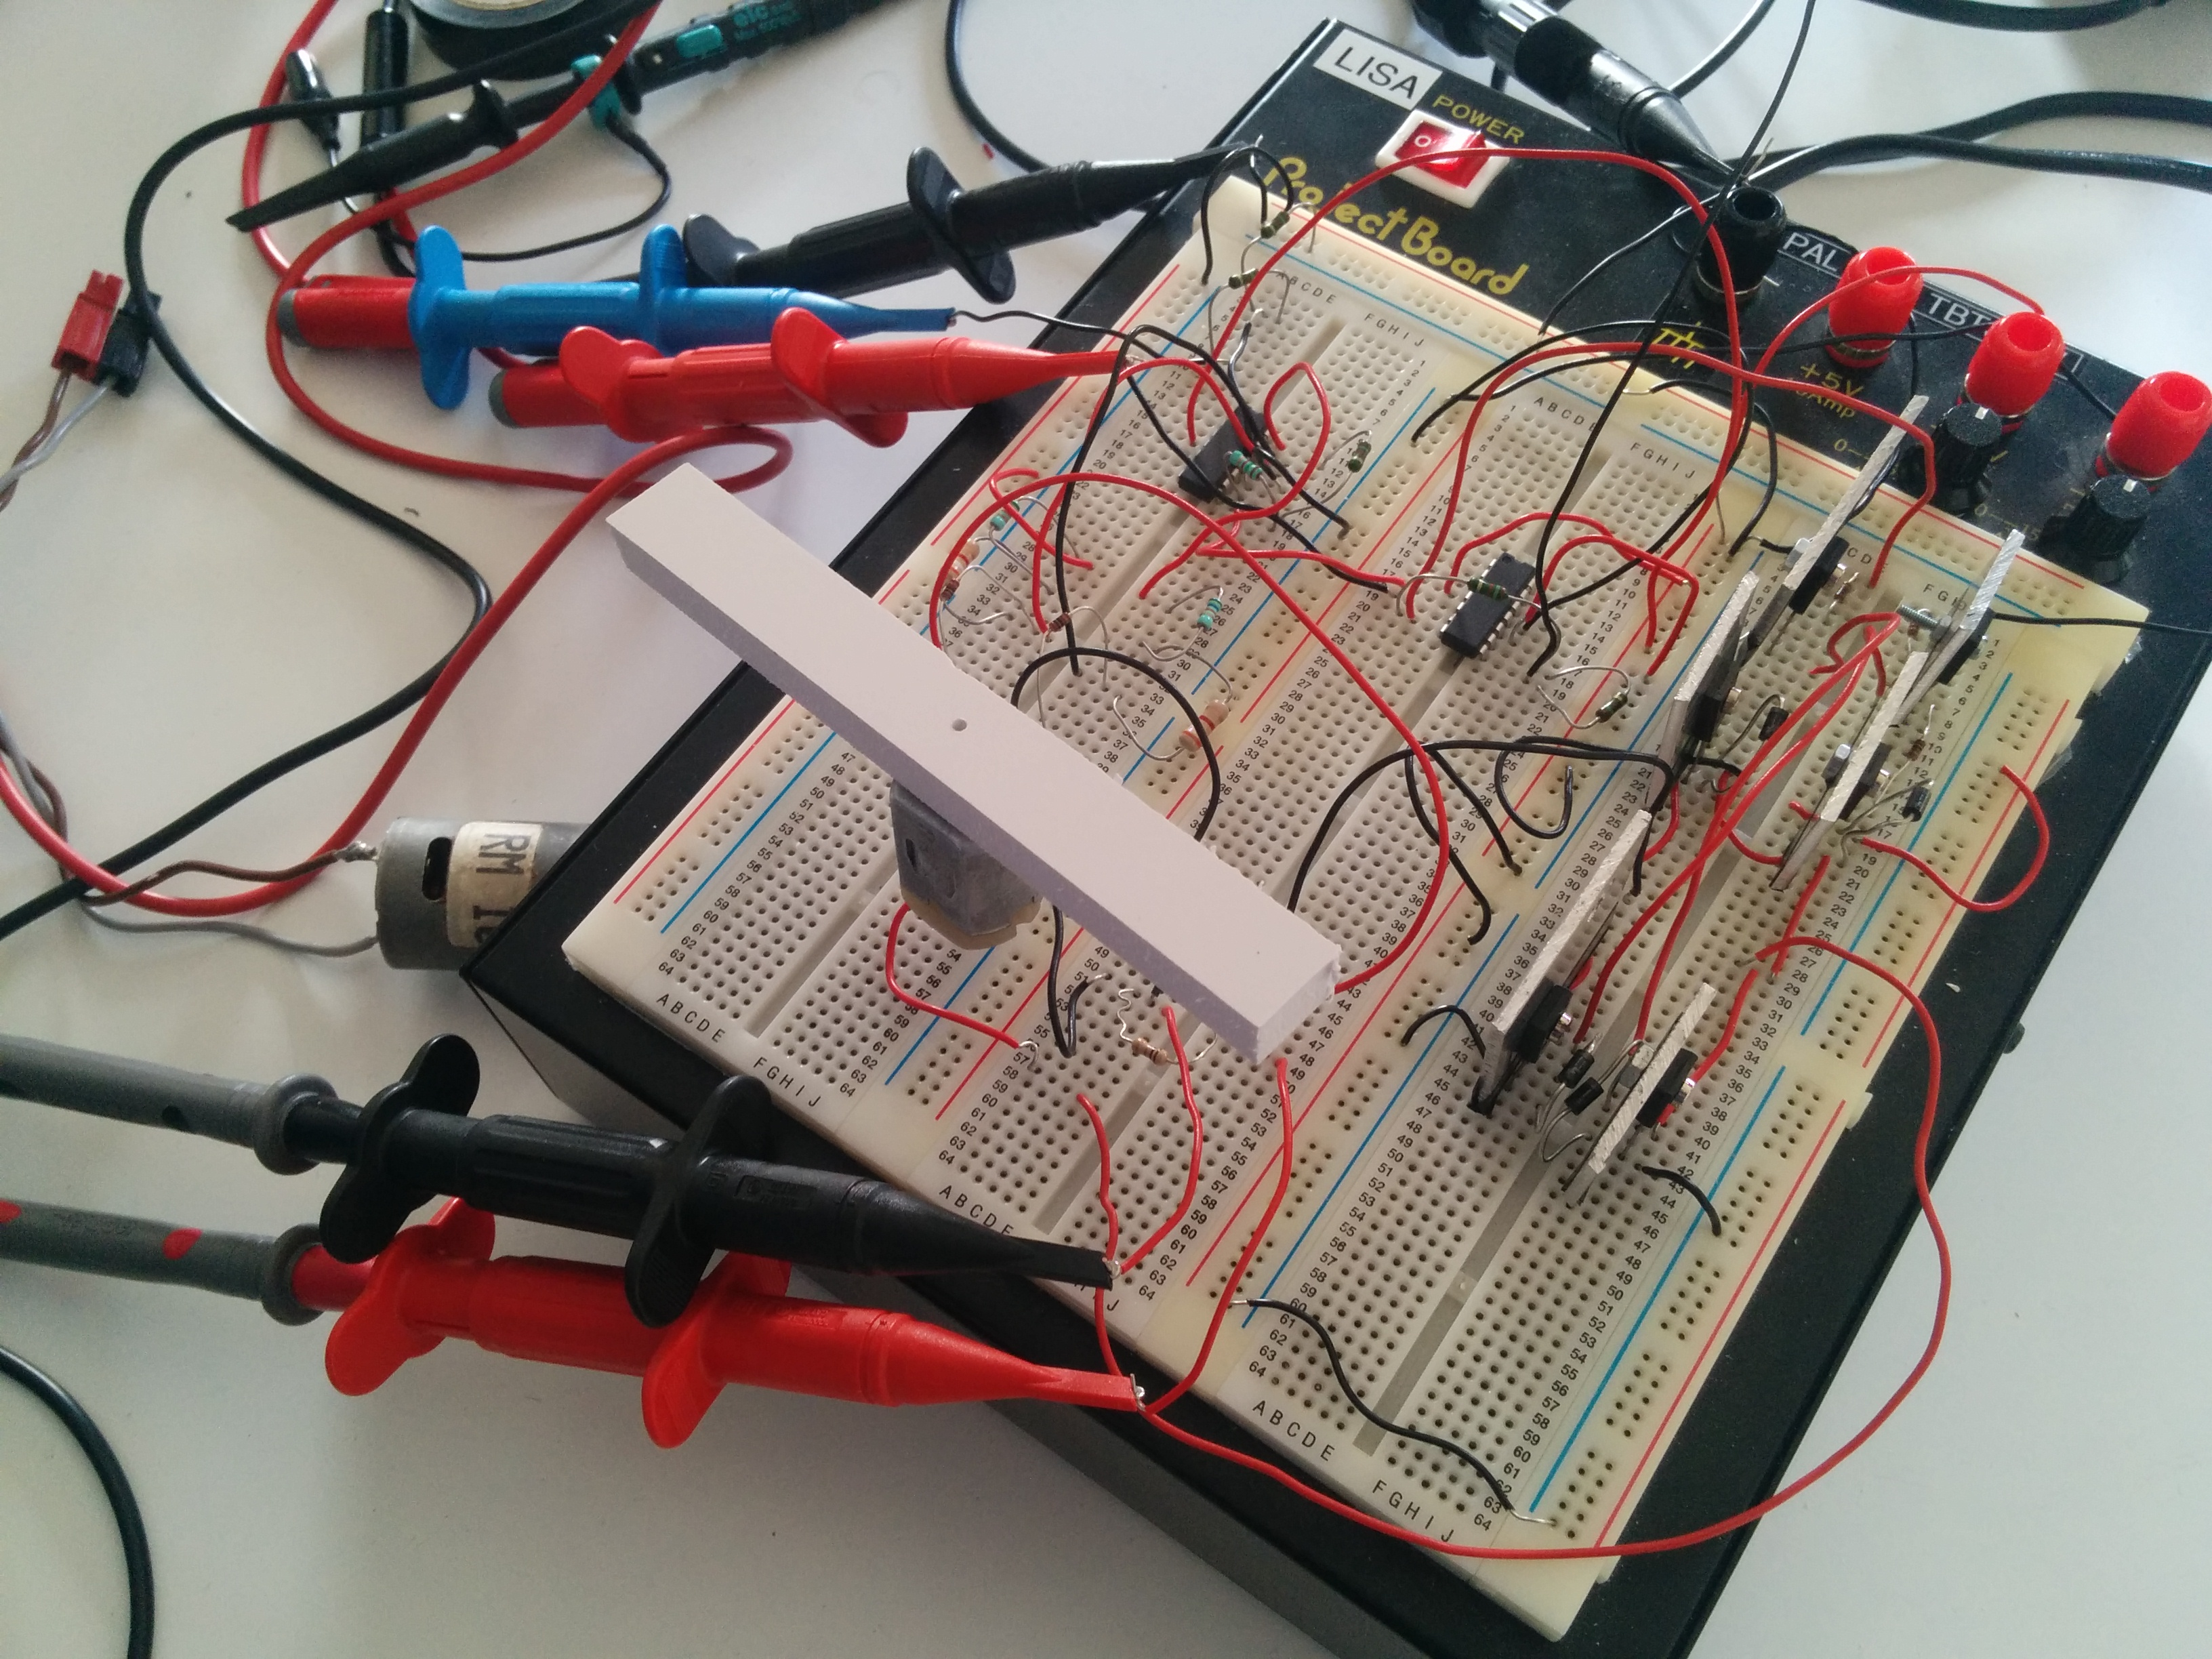
\includegraphics[width=1\textwidth]{circuit}
  \caption{Le circuit réalisé}
\end{figure}

\subsection{Résultats}

Les résultats sont expliqués dans la vidéo de présentation. Voici quelques screenshots d'oscilloscope illustrant les entrées du pont en H et la tension imposée au moteur.

\begin{figure}[H]
  \centering
    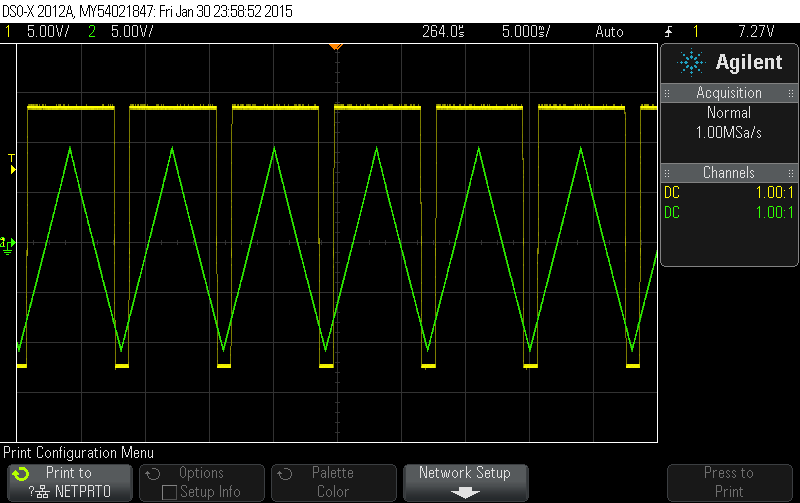
\includegraphics[width=1\textwidth]{scope_1}
  \caption{Entrée positive du pont en H}
\end{figure}

\begin{figure}[H]
  \centering
    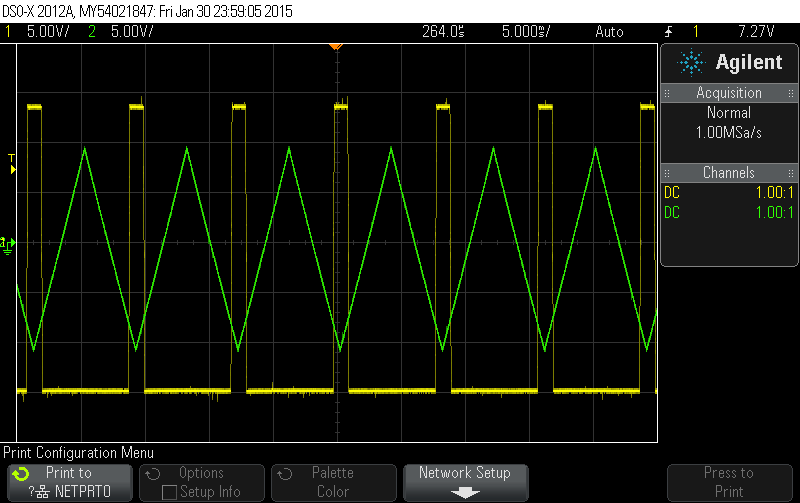
\includegraphics[width=1\textwidth]{scope_2}
  \caption{Entrée négative du pont en H}
\end{figure}

\begin{figure}[H]
  \centering
    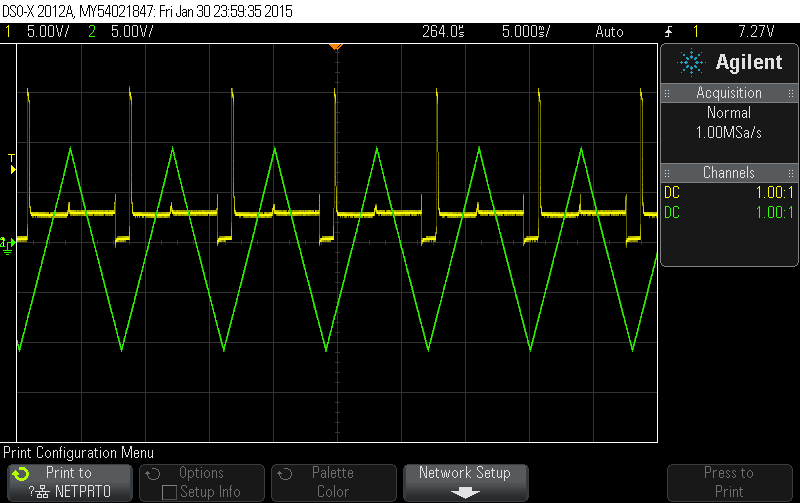
\includegraphics[width=1\textwidth]{scope_3}
  \caption{Tension aux bornes du moteur}
\end{figure}


\end{document}